%\documentclass[12pt,parskip=half]{scrartcl}
\documentclass{TechReport}

% Select Sans serif font "Computer Modern Bright"
%\usepackage[T1]{fontenc}
%\usepackage{cmbright}

% ***TODO*** Select the right encoding for your document
%\usepackage[utf8]{inputenc}
%\usepackage[latin1]{inputenc}

%\usepackage{graphicx}

% Bibtex citation package
%\usepackage{cite}

%\usepackage{url}

% No page numbers here; these will be added for final Tech Report with
% all contributions
%\renewcommand*{\titlepagestyle}{empty}
%\pagestyle{empty}

%\title{LaTeX-Template for a Technical Report}
%\author{Christian Bockermann}
\date{01/2012}  % Serial Number/Year
\sfbproject{C3} % Your project identifier (two digit version)

\usepackage{amssymb}
\usepackage{afterpage}


% ***TODO*** Choose correct title, author, department and email address
\title{\vspace{6ex}The \textsf{streams} Framework \\*[1ex] {\large Version 0.9.6}}
\author{{\large Christian Bockermann and Hendrik Blom\\*[1ex]
  Lehrstuhl f\"ur k\"unstliche Intelligenz\\
  Technische Universit\"at Dortmund\\*[1ex]
  {\ttfamily firstname.lastname@udo.edu}}}
% Please keep date empty
\date{}





\usepackage{listings}
\usepackage{hyperref}
\hypersetup{
  linktoc=all
}

\usepackage{tikz}
\usetikzlibrary{shapes} 
\usetikzlibrary{decorations,arrows} 
\usetikzlibrary{decorations.pathmorphing} 
\usepgflibrary{decorations.pathreplacing} 

\usepackage{algorithm}
%\usepackage{algorithmicx}
\usepackage{algpseudocode}
\usepackage{tocvsec2}
\usepackage{color}
\definecolor{rapidi}{RGB}{240,176,0}
\definecolor{rapidiText}{RGB}{102,51,0}
\definecolor{darkGreen}{RGB}{67,101,0}

\DeclareRobustCommand{\pointer}[1]{\tikz\node[draw,circle,draw=darkGreen,thick,fill=darkGreen!70,inner sep=1pt] at (0,-0.1) {\scriptsize\color{white}\textsf{#1}};} 

\lstset{language=XML,
%  otherkeywords={stream,container,process,service},
  basewidth={0.5em,0.45em},
  fontadjust=false,
  basicstyle=\footnotesize\ttfamily,
  keywordstyle=\color{blue},          % keyword style
  commentstyle=\ttfamily\color{black!60},       % comment style
  stringstyle=\color{darkGreen}
}

\lstdefinelanguage{JavaScript}{
  keywords={typeof, new, true, false, catch, function, return, null, catch, switch, var, if, in, while, do, else, case, break},
  keywordstyle=\color{blue}\bfseries,
  ndkeywords={class, export, boolean, throw, implements, import, this},
  ndkeywordstyle=\color{darkgray}\bfseries,
  identifierstyle=\color{black},
  sensitive=false,
  comment=[l]{//},
  morecomment=[s]{/*}{*/},
  commentstyle=\color{purple}\ttfamily,
  stringstyle=\color{red}\ttfamily,
  morestring=[b]',
  morestring=[b]"
}

%\newcommand{\todo}[1]{\marginpar{{\bf TODO:}\\#1}}
%\newcommand{\TODO}[1]{{{\bf TODO:} #1}}
\newcommand{\todo}[1]{}
\newcommand{\TODO}[1]{}
\newcommand{\baustelle}{\marginpar{
  
\includegraphics[scale=0.2]{graphics/construction.png}}}

\newcommand{\streams}{{\em streams}\ }
\newcommand{\rapidminer}{{\footnotesize\textsf{RapidMiner}\ }}
\newcommand{\plugin}{{\em Streams Plugin}}

\newcommand{\defitem}[1]{\item[{\footnotesize\textbf{\textsf{#1}}}]}
\newcommand{\bigO}{\cO}
\newcommand{\barw}{\bar{w}}
\newcommand{\barbarw}{\bar w_M^\circ}
\newcommand{\vx}{x}

\newcommand{\sample}[1]{
{\centering
\begin{tikzpicture}[
  auto, every node/.style= { text width=0.8\textwidth},
  block/.style = {rectangle, draw=black!40, thick, fill=black!8, inner sep=1ex, minimum width=0.9\textwidth,
                  rounded corners=1.25pt}]
\node [block,anchor=west] (titel) at (0,0) {\ttfamily #1 \hfill};
\end{tikzpicture}}
}

\newenvironment{xml}{\begin{figure}[h!]
   \begin{lstlisting}{lang=xml}}{\end{lstlisting}
\end{figure}
}



\input{streams.pkg}

\setcounter{tocdepth}{4} %to make it appears in TOC
\setcounter{secnumdepth}{4} %to make it numbered

\begin{document}

\makesfbtitlepage

\newpage
\tableofcontents
\cleardoublepage
\ 
\newpage

\part{The {\em streams} Framework}

\begin{abstract}
{\normalsize
  In this report, we present the \streams library, a generic
  Java-based library for designing data stream processes. The \streams
  library defines a simple abstraction layer for data processing and
  provides a small set of online algorithms for counting and
  classification. Moreover it integrates existing libraries such as
  MOA. Processes are defined in XML files following the
  semantics and ideas of well established tools like Ant, Maven or the
  Spring Framework.

  The \streams library can be easily embedded into existing software,
  used as a standalone tool or be used to define compute graphs that
  are executed on other backend systems such as the Storm stream
  engine.
}

\medskip 

{\normalsize This report reflects the status of the \streams framework
  in version 0.9.6. As the framework is continuously enhanced, the
  report is extended along. The most recent version of this report is
  available online\footnote{The latest version of the report is
    available at
    \url{http://www.jwall.org/streams/tr.pdf}.}. \baustelle }
\end{abstract}


%%
%% Section 1 Introduction
%%
\section{\label{sec:intro}Introduction}
In toddy's applications, data is continuously produced in various spots
ranging from network traffic, log file data, monitoring of
manufacturing processes or scientific experiments. The applications
typically emit data in non-terminating data streams at a high rate,
which poses tight challenges on the analysis of such streams.

We illustrate this by projects of our Collaborative Research Center
SFB-876. A first example is given by the FACT telescope that is
associated to project C3. This telescope observes cosmic showers by
tracking light that is produced by these showers in the atmosphere
with a camera.  These showers last about 20 nanoseconds and are
recorded with a camera of 1440 pixels at a sampling rate of 2 GHz. As
about 60 of these showers are currently recorded each second, a
5-minute recording interval quickly produces several gigabytes of raw
data.

Other high-volume data is produced in monitoring system behavior, as
performed in project A1. Here, operating systems are monitored by
recording fine grained logs of system calls to catch typical usage of
the system and optimize its resource utilization (e.g. for energy
saving). System calls occur at a high rate and recording produces a
plethora of log entries.

The project B3 focuses on monitoring (distributed) sensors in an
automated manufacturing process. These sensors emit detailed
information of the oven heat or milling pressure of steel production
and are recorded at fine grained time intervals. Analysis of this data
focuses on supervision and optimization of the production process.

\subsubsection*{From Batches to Streams}
The traditional batch data processing aims at computations on fixed
chunks of data in one or more passes. Such data is usually stored in
files or database systems providing random access to each record. The
results of these computations again form a fixed outcome that can
further be used as input. A simple example is given by the computation
of a prediction model based on some fixed set of training data. After
the determination of a final model, the learning step is finished and
the model is applied to deliver predictions based on the learning
phase. Similar situations arise for the computation of statistics,
creation of histograms, plots and the like. From a machine learning
perspective, this has been the predominant approach of the last years.

Two fundamental aspects have changed in the data we are facing today,
requiring a paradigm shift: The size of data sets has grown to amounts
intractable by existing batch approaches, and the rate at which data
changes demands for short-term reactions to data drifts and updates of
the models.

%\subsubsection*{Processing Masses of Data}
The problem of big data has generally been addressed by massive
parallelism. With the drop of hardware prizes and evolving use of
large cloud setups, computing farms are deployed to handle data at a
large scale. Though parallelism and concepts for cluster computing
have been studied for long, their applicability was mostly limited to
specific use cases.

One of the most influential works to use computing clusters in data
analysis is probably Google's revival of the {\em map-and-reduce}
paradigm \cite{googleMapReduce}. The concept has been around in
functional programming for years and has now been transported to
large-scale cluster systems consisting of thousands of compute
nodes. Apache's open-source {\em Hadoop} implementation of a
map-and-reduce platform nowadays builds a foundation for various
large-scale systems.

With the revival of map-and-reduce, various machine learning algorithms
have been proven to be adjustable to this new (old) way of computing.

\subsection{\label{sec:streamSetting}The Problem of Continuous Data}
Whereas the massive parallelism addresses the batch computation of
large volumes of data, it still requires substantial processing time
to re-compute prediction models, statistics or indexes once data has
changed. Therefore it does not fully reflect the demands for reacting
to short-term drifts of data.

Within this work we will refer to this as the setting of {\em
  continuous data}, i.e. we consider an unbound source $D$ of data
that continuously emits data items $d_i$. In the following, we model
that data stream as a sequence
$$D = \langle d_0,d_1,\ldots,d_i,\ldots \rangle$$
with $i\rightarrow\infty$. The framing to operate on streaming data is
generally given by the following constraints/requirements:
\begin{itemize}
  \defitem{C1} continuously processing {\em single items} or {\em small batches} of data,
  \defitem{C2} using only a {\em single pass} over the data,
  \defitem{C3} using {\em limited resources} (memory, time),
  \defitem{C4} provide {\em anytime services} (models, statistics).
\end{itemize}


To catch up with the requirements of large scale and continuous data,
online algorithms have recently received a lot of attention. The focus
of these algorithms is to provide approximate results while limiting
the memory and time resources required for computation. 
%The
%constraints for the data stream setting are generally defined by
%allowing only a single pass over the data, and focusing on
%approximation schemes to deal with the inbalance of data volume to
%computing resources. In addition, models computed on streaming data
%are expected to be queriable at any time.


\subsubsection*{Analysis of Continuous Data}
%{\bf TODO: \"{U}berleitungssatz?}
Traditional data analysis methods focus on processing fixed size
batches of data and often require the data (or large portions of it)
to be available in main memory. This renders most approaches useless
for continuously analyzing data that arrives in steady streams. Even
procedures like preprocessing or feature extraction can quickly become
challenging for continuous data, especially when only limited
resources with respect to memory or computing power are available.

At any time $t$ we want to provide some model that reflects the
analysis of the items $d_i$ with $i\le t$.  Typical analysis tasks to
compute on $S$ are
\begin{itemize}
\item Given $d_i \in \mathbb{N}$ - finding the top-$k$ most frequent
  values observed until $t$.
\item For $d_i \in \mathbb{N}^p$ - find the item sets $I \subset
  \mathbb{N}^p$ which most frequently occurred in the $d_i$.
\item With $d_i \subset X$, provide a classifier $c:X \rightarrow Y$,
  that best approximates the real distribution of labeled data $X
  \times Y$ (classification).
\item Provide a clustering $C$ for the data item $d_i$ observed so far (clustering).
\item Find indications on when the overall distribution of the $d_i$
  changes within the stream (concept drift detection).
\end{itemize}
Often, these tasks are further refined to models that focus on a
recent sliding window of the last $w$ data items observed, e.g. we are
interested in the top-$k$ elements of the last 5 minutes. 

Algorithms for solving these tasks on static data sets
exists. However, the challenging requirements in the continuous data
setting are the tight limits on the resources available for
computation. This can for example be real-time constraints, such as a
fixed limit on the time available for processing a data item, or a
bound on the memory available for computation.

Various algorithms have been proposed dedicated to computational
problems on data streams. Examples include online quantile computation
\cite{Greenwald/Khanna/2001a,Arasu/Manku/2004a}, distinct counting of
elements, frequent item set mining
\cite{Charikar02findingfrequent,goethals2007,Cheng06maintainingfrequent},
clustering \cite{sohler2010,Aggarwal:2003} or training of classifiers
on a stream \cite{Domingos/Hulten/2000a}.

Here, we want to provide an abstract framework for putting online
learning algorithms to good use on data streams.

\subsection{Designing Stream Processes}

%\subsection*{Existing Frameworks}
%Various frameworks exist that support either of these two processing
%modes.
Parallel batch processing is addressing the setting of fixed data and
is of limited use if data is non-stationary but continuously produced,
for example in monitoring applications (server log files, sensor
networks).  A framework that provides online analysis is the MOA
library \cite{moa}, which is a Java library closely related to the
WEKA data mining framework \cite{weka}. MOA provides a collection of
online learning algorithms with a focus on evaluation and
benchmarking.

Aiming at processing high-volume data streams two environments have
been proposed by Yahoo! and Twitter. Yahoo!'s {\em S4} \cite{s4io} as
well as Twitter's {\em Storm} \cite{storm} framework do provide online
processing and storage by building on large cluster infrastructures such
as Apache's Zookeeper infrastructure.

The {\em Storm} engine relies on executing a computing graph, called a
{\em topology} in Storm. The nodes (referred to as {\em Bolts}) in this
graph are user written programs defining the data processing
steps. The topology is then provided by the user by implementing a
Java program that creates the desired topology (a {\em topology
  builder}). To start the topology, the custom topology builder
implemented by the user is given to the storm engine, which creating
the bolts and distributing it along the cluster infrastructure.

While the {\em Storm} engine is known to be fast and scalable, it
requires an in-depth knowledge of the user on how to create a topology
that matches a particular task. Looking from the perspective of a {\em
  data analyst}, this does not match the higher-level
rapid-prototyping needs as is adequate for domain experts e.g. in
projects like telescope data analysis mentioned above.


\TODO{More about User/Developer roles, abstraction levels and toolkit
  building blocks.}

In contrast to these frameworks, the \streams library focuses on
defining a simple abstraction layer that allows for the definition of
stream processes by means of only a few basic conceptual elements.
The resulting processes can be then be easily executed by the \streams
run-time or mapped to different run-time environments such as {\em S4}
or {\em Storm}.

\subsubsection*{Our Contributions}
In this work we introduce the \streams library, a small software
framework that provides an abstract modeling of stream processes. The
objective of this framework is to establish a layer of abstraction
that allows for defining stream processes at a high level, while
providing the glue to connect various existing libraries such as MOA
\cite{moa}, WEKA \cite{weka} or the RapidMiner tool.

The set of existing online algorithms provides a valuable collection
of algorithms, ideas and techniques to build upon. Based on these core
elements we seek to design a process environment for implementing
stream processes by combining implementations of existing online
algorithms, online feature extraction methods and other preprocessing
elements.
%or implement and evaluate custom online algorithms 

Moreover it provides a simple programming API to implement and
integrate custom data processors into the designed stream processes.
The level of abstraction of this programming API is intended to
flawlessly integrate into existing run-time environments like {\em
  Storm} or the RapidMiner platform \cite{rapidminerStreams}.

Our proposed framework supports
\begin{enumerate}
\item Modeling of continuous stream processes, following the {\em
    single-pass} paradigm,
\item Anytime access to services that are provided by the modeled
  processes and the online algorithms deployed in the process setup,
  and
\item Processing of large data sets using limited memory resources
\item A simple environment to implement custom stream processors and
  integrate these into the modeling
\item A collection of online algorithms for counting and classification
\item Incorporation of various existing libraries (e.g. MOA
  \cite{moa}) into the modeled process.
\end{enumerate}

The rest of this report is structured as follows: In Section
\ref{sec:abstraction} we derive a set of basic building blocks for the
abstract modeling data stream processes. In Section
\ref{sec:processDesign} we present the XML based definition language
and several addition concepts that allow for designing stream
processes within the framework. Based on this we outline two example
use-cases for processing and analyzing streaming data with the
\streams library. Finally we summarize the ideas behind the \streams
library and give an outlook on future work in Section
\ref{sec:summary}. A comprehensive description of the implementations
and guides for setting up a standalone processing environment provided
by our framework is given in the appendix.


\newpage
%%
%% Section 2 Abstract Processing Model
%%
%%
%% Structure of this section
%%
%%  3.1 define basics, abstraction of stream processing
%%    - Def. data items, data streams,...
%%    - data flow vs. control flow => Bezug zu Anytime
%%    - Warum keine "Meta-Daten" (bisher)
%%
%%  3.2 Umsetzung/Modellierung in Form der Stream-API
%%    - Abbildung der Konzepte aus 3.1 auf "Java Welt"
%%  
%%  3.3 Example Runtime for RapidPrototyping, Debugging
%%    + Ausblick auf section 4 => streamplugin + runtime für RapidMiner
%%
%%
\clearpage
\section{\label{sec:abstraction}An Abstract Stream Processing Model}
Processing streaming data can generally be viewed as establishing a
{\em data flow graph} where each of the nodes of the graph corresponds
to some function that is applied as data is passed along the
edges. This general idea can be found in various existing approaches
built on top of message passing systems and has been adopted by
streaming systems such as SPADE, Kafka or Storm.

As the existing systems, the \streams framework is based on an
abstract definition of such data flow graphs, following the {\em
  pipes-and-filters} pattern \cite{softwarePatterns}. To that it adds
an additional {\em control flow} view, which allows for the
implementation of systems fulfilling the anytime requirement as
described in Section \ref{sec:intro}. Figure \ref{fig:xmlProcess}
outlines a general data flow graph built from elements like {\em
  streams} (S), {\em processes} (P) and {\em queues} (Q) and
additional control flow elements represented by {\em services} shown
in orange color.

\begin{figure}[b!]
  \centering
  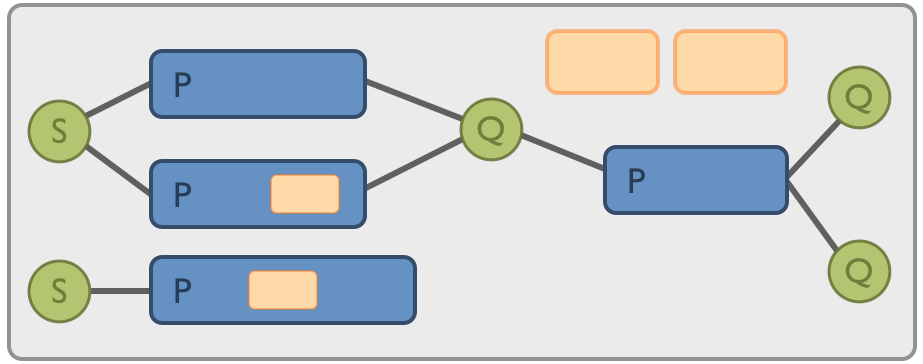
\includegraphics[scale=0.3]{graphics/streams-graph}
  \caption{\label{fig:xmlProcess} The general concept of a data-flow
    graph. The \streams framework provides means for defining streams
    (S), connected processes (P), queues (Q) and adds an abstract
    orthogonal control flow layer (orange elements).}
\end{figure}

In this section we introduce the basic concepts and ideas that we
model within the \streams framework. This mainly comprises the data
flow), the control flow (anytime services) and the basic data
structures and elements used for data processing. The objective of the
abstraction layer is to provide a simple means for rapid prototyping
of data stream processes and a clean and easy-to-use API to implement
against.

The structure of the \streams framework builds upon three aspects:
\begin{enumerate}
\item A {\em data representation} which provides a modeling of the
  data that is to be processed by the designed stream processes
\item Elements to model a {\em data flow}
\item A notion of {\em services} which allow for the implementation
  of {\em anytime service} capabilities.
\end{enumerate}
All of these elements are provided as simple facades (interfaces)
which have default implementations. The abstraction layer provided by
these facades is intended to cover most of the use cases with its
default assumptions, whereas any special use cases can generally be
modeled using a combination of different building blocks of the API
(e.g. queues, services) or custom implementations of the facades.

\subsection*{\label{sec:xmlToRuntime}Executing Data Flow Graphs}
The main objective of the \streams framework is to provide an adequate
abstraction layer, which enables users to design streaming processes
without the need to write any code. A user can prototype {\em
  containers}, which are the top-level elements containing a data flow
graph built from the base elements {\em stream}, {\em process} and
{\em queues}. The {\em process} elements are the executing instances
which need to be enriched with functions ({\em processors}) that do
the actual work. The framework provides a large set of such processors
that can be used to add the required functionality into the data flow
graph. The containers (graphs) are defined in XML.

The XML process definitions are designed to be independent of the
underlying execution platform. The \streams framework provides its own
default runtime implementation, which is able to execute the XML data
flow graphs. This {\em streams} runtime is a Java library with a very
small footprint (less than 200 kilobytes) that can be instantly executed on any
Java VM.

In addition, \streams provides a compiler to map XML process
definitions to {\em Storm} topology, to execute processes on a Storm
cluster. A third execution engine is provided for the Android
platform, which allows for running \streams definitions on mobile
devices that are powered by the Android operating system.\baustelle


\begin{figure}[h!]
  \centering
  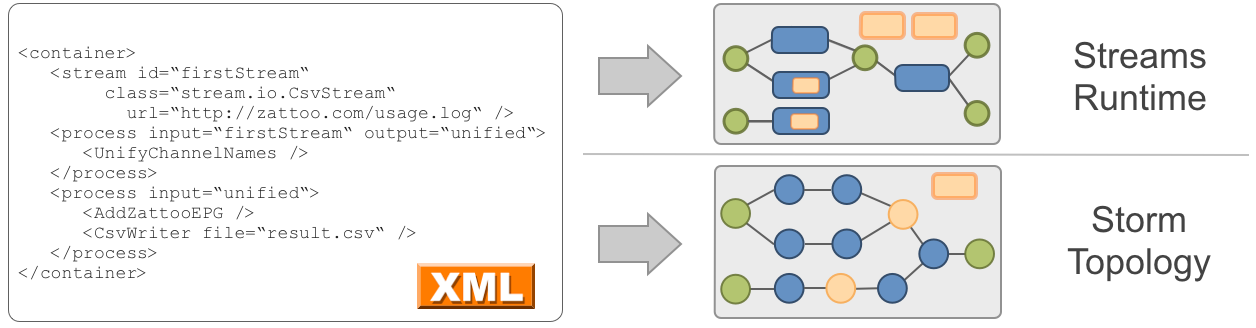
\includegraphics[scale=0.3]{graphics/compile-xml}
  \caption{\label{fig:compileXml}The XML is compiled into a data flow
    graph for different runtime environments. Currently the \streams
    runtime is supported and a prototype for the {\em Storm} compiler
    exists.}
\end{figure}


\subsection{\label{sec:data}Data Representation and Streams}
A central aspect of data stream processing is the representation of
data items that contain the values which are to be processed. From a
message passing system point of view this is the concrete
representation of messages. The abstraction of the \streams framework
considers the case of continuous streaming data being modeled as a
sequence of {\em data items} which traverse the compute graph.

A data item is a set of $(k,v)$ pairs, where each pair reflects
an attribute with a name $k$ and a value $v$. The names are required
to be of type {\ttfamily String} whereas the values can be of any
type that implements Java's {\ttfamily Serializable} interface. The
data item is provided by the {\ttfamily stream.Data} interface.

\begin{table}[h!]
\centering
{
\renewcommand{\arraystretch}{1.25}
\begin{tabular}{c|c}\hline
\textsf{\textbf{Key}} & \textsf{\textbf{Value}} \\ \hline \hline
{\ttfamily x1} & {\ttfamily 1.3} \\ \hline
{\ttfamily x2} & {\ttfamily 8.4} \\ \hline
{\ttfamily source} & {\ttfamily "file:/tmp/test.csv"}  \\ \hline
\end{tabular}
}
\caption{\label{tab:dataitem}A data item example with 3 attributes.} 
\end{table}

Table \ref{tab:dataitem} shows a sample data item as a table of
(key,value) rows. This representation of data items is provided
by hash tables, which are generally provided in almost every modern
programming language.

The use of such hash tables was chosen to provide a flexible data
structure that allows for encoding a wide range of record type as well
as supporting easy interoperation when combining different programming
languages to implement parts of a streaming process. This enables the
use of languages like Python, Ruby or JavaScript to implement custom
process as we will outline in more detail in Section
\ref{sec:scripting}.

\subsection*{Streams of Data}
A {\em data stream} in consequence is an entity that provides access
to a (possibly unbounded) sequence of such data items. Again, the
\streams abstraction layer defines data streams as an interface, which
essentially provides a method to obtain the next item of a stream.

\begin{figure}[h1]
  \begin{center}
    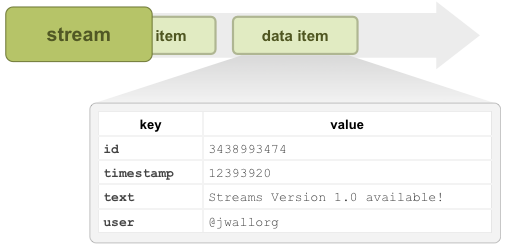
\includegraphics[scale=0.5]{graphics/stream-items.png}
  \end{center}
  \caption{\label{fig:datastream}A {\em data stream} as a sequence of {\em data item} objects.}
\end{figure}

The core \streams library contains several implementations for data
streams that reveal data items from numerous formats such as CSV data,
SQL databases, JSON or XML formatted data. A list of the available
data stream implementations is available in the appendix \ref{app:dataStreams}.

In addition, application specific implementations for data streams can
easily be provided by custom Java classes, as is the case in the FACT
telescope data use-case outlined in section \ref{sec:fact}.

%Throughout this work, we will denote a {\em
%  data stream} by $D$ and a family of such streams as $D_l$. A data
%stream $D$ is a sequence
%\begin{displaymath}
%  D = \langle d_0,d_1,\ldots,d_i,\ldots \rangle
%\end{displaymath}
%of data items $d_i$. Let $A = \{A_1,\ldots,A_p\}$ be a set of
%attributes, then a data item $d_i$ is a function mapping attributes to
%values of a domain associated with each attribute. In database
%notation, each $d_i$ is a tuple of $M^p = M_{A_1} \times\ldots\times
%M_{A_p}$ for sets $M_j$. The $M_j$ can be any discrete sets of a fixed
%domain as well as $M_j \subseteq \mathbb{R}$. The values of each data
%item are further denoted by $d_i(k)$, i.e.
%\begin{displaymath}
%  d_i = ( d_i(A_1),\ldots,d_i(A_p) ).
%\end{displaymath}
%
%The index $i$ may reflect some time unit or a (monotonically
%increasing) time-like dimension, constituting the sequence of
%tuples. For $p=1$ and $M_1 = \mathbb{R}$ this models a single value
%series with index $i$.


%
%. The {\em data items} $s_i$ are tuples of
%$M^p$ with $p \ge 1$ where $M^p = M_1 \times \ldots \times M_p$ for
%any sets $M_j$. 
%

\subsection{\label{sec:basics}Processes and Processors}
The {\em data stream}s defined above encapsulate the format and reading
of data items from some source. The \streams framework defines a
{\em process} as the consumer of such a source of items. A process is
connected to a stream and will apply a series of {\em processors} to
each item that it reads from its attached data stream.

Each {\em processor} is a function that is applied to a data item and
will return a (modified or new) data item as a result. The resulting
data item then serves as input to the next processor of the
process. This reflects the pipes-and-filters concept mentioned in the
beginning of this section.

The {\em processors} are the low-level functional units that actually
do the data processing and transform the data items. There exists a
variety of different processors for manipulating data, extracting or
parsing values or computing new attributes that are added to the data
items.  From the perspective of a process designer, the {\em stream}
and {\em process} elements form the basic data flow elements whereas
the processors are those that do the work.

\begin{figure}[h!]
\centering
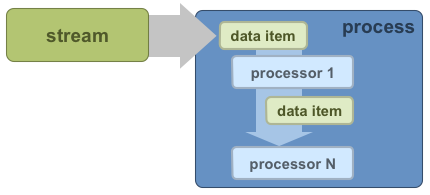
\includegraphics[scale=0.5]{graphics/inside-process.png}
\caption{\label{fig:process}A process reading from a stream and applying processors.}
\end{figure}

The simple setup in Figure \ref{fig:process} shows the general role of
a process and its processors. In the default implementations of the
\streams library, this forms a {\em pull oriented} data flow pattern
as the process reads from the stream one item at a time and will only
read the next item if all the inner processors have completed. 

Where this pull strategy forms a computing strategy of {\em lazy
  evaluation} as the data items are only read as they are processed,
the \streams library is not limited to a {\em pull oriented} data
flow.
% We discuss the implementation of {\em active streams} and the
%resulting {\em push} oriented data flow in Section \ref{sec:push}.


\subsection*{Using multiple Processes}
In the \streams framework, processes are by default the only executing
elements. A process reads from its attached stream and applies all
inner processors to each data item. The process will be running until
no more data items can be read from the stream (i.e. the stream
returns {\ttfamily null}). Multiple streams and processes can be
defined and executing in parallel, making use of multi-core CPUs as
each process is run in a separate thread\footnote{This is the default
  behavior in the reference \streams runtime implementation. If
  \streams processes are executed in other environments, thus behavior
  might be subject to change.}.

For communication between processes, the \streams environment provides
the notion of {\em queues}. Queues can temporarily store a limited
number of data items and can be fed by processors. They do provide
stream functionality as well, which allows queues to be read from by
other processes.

Figure \ref{fig:queues} shows two processes being connected by a
queue. The enlarged processor in the first process is a simple {\em
  Enqueue} processor that pushes a copy of the current data item into
the queue of the second process. The second process constantly reads
from this queue, blocking while the queue is empty.

\begin{figure}[h!]
  \begin{center}
    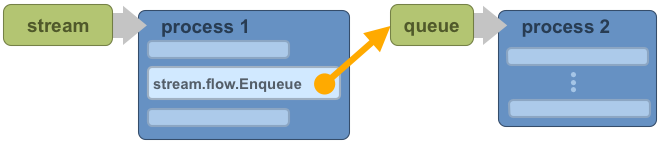
\includegraphics[scale=0.5]{graphics/process-queues.png}
  \end{center}
  \caption{\label{fig:queues}Two Processes $P_1$ and $P_2$ communicating via queues.}
\end{figure}

\bigskip

These five basic elements ({\em stream}, {\em data item}, {\em
  processor}, {\em process} and {\em queue}) already allow for
modeling a wide range of data stream processes with a sequential and
multi-threaded data flow. Apart from the continuous nature of the data stream source, this model
of execution matches the same pipelining idea known from tools like
RapidMiner, where each processor (operator) performs some work on a
complete set of data (example set).
%This contrasts to the current RapidMiner execution model, where each
%operator within a process is executed only once (not counting loops as
%within a cross validation).
%This simple {\em data flow} view serves as the basic data-driven
%exectuion model. 

\subsection{Data Flow and Control Flow}
A fundamental requirement of data stream processing is given by the
{\em anytime paradigm}, which allows for querying processors for their
state, prediction model or aggregated statistics at any time. We will
refer to this anytime access as the {\em control flow}.  Within the
\streams framework, these anytime available functions are modeled as {\em
  services}. A service is a set of functions that is usually provided
by processors and which can be invoked at any time. Other processors
may consume/call services. 

This defines a control flow that is orthogonal to the data flow. Whereas
the flow of data is sequential and determined by the data source, the
control flow represents the anytime property as the functions of services
may be called asynchronous to the data flow.
Figure \ref{fig:control} shows the flow of data and service access.

Examples for services my be classifiers, which provide functions for
predictions based on their current state (model); static lookup
services, which provide additional data to be merged into the stream
or services that can be queried for current statistical information
(mean, average, counts).

\begin{figure}[h!]
  \begin{center}
    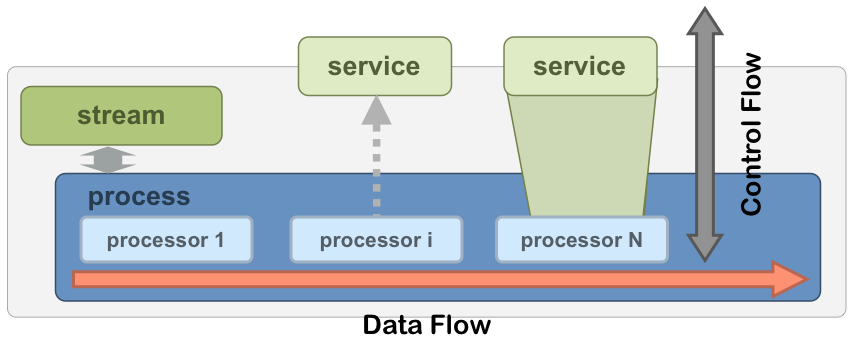
\includegraphics[scale=0.35]{graphics/data-control-flow.png}
  \end{center}
  \caption{\label{fig:control}Orthogonal {\em data} and {\em control
      flow}. Processors may use services as well as export
    functionality by providing services.}
\end{figure}

\subsubsection*{Service References and Naming Scheme}
In order to define the data flow as well as the control flow, a naming
scheme is required. Each service needs to have an unique identifier assigned
to it. This identifier is available within the scope of the experiment and
will be used by service consumers (e.g. other processors) to reference that
service.

At a higher level, when multiple experiments or stream environments are running
in parallel, each experiment is associated with an identifier by itself. This
imposes a hierarchical namespace of experiments and services that are defined
within these experiments. The {\em streams} library constitutes a general
naming scheme to allow for referencing services within a single experiment
as well as referring to services within other (running) experiments.

A simple local reference to a service or other element (e.g. a queue) is 
provided by using the identifier (string) that has been specified along with
the service definition. Following a URL like naming format, services within
other experiments can be referenced by using the experiment identifier and
the service/element identifier that is to be referred to within that experiment,
e.g.
\begin{displaymath}
  \mbox{\ttfamily //experiment-3/classifier-2}.
\end{displaymath}
Such names will be used by the \streams library to automatically resolve references
to services and elements like queues.




%
%
%\subsection{Service Registration and Lookup}
%Each service defined within a process needs to have an unique
%identifier assigned to it. This identifier is used to reference that
%service, e.g. from a processor.

%%It is also possible to define standalone services, e.g. for lookup
%%tables on static data. Processors may also consume services.  
%%\subsubsection*{Using Services for Test-then-Train Evaluation}
%A simple example is given by a learning algorithm (classifier). This
%can process data items as part of its learning process. It provides a
%{\em PredictionService}, which contains as single {\ttfamily predict}
%function. This function uses the current prediction model of the
%learning algorithm to return a prediction for a data item. 

%Figure \ref{fig:control} shows the {\em Naive Bayes Learner} embedded
%into a process. This process implements the {\em test-then-train}
%methods for evaluating stream classifiers on labeled data
%streams. Each item of the stream is first used for testing by making a
%prediction for that item, and then used for updating the prediction
%model.

%The first processor {\em Add Prediction} in this process uses the
%prediction service provided by the {\em Naive Bayes Learner} to make
%a prediction for each data item. After the prediction, the item is
%handed over to the learner, which incorporates it into its model.

%After these two processors, the data item contains the original, true
%label, and the prediction added by the {\em Add Prediction} processor.
%The {\em Prediction Error} processor can now apply any loss function
%to determine the prediction error and aggregate that error over time.

%\subsection{Multiple Processes}
%Often, applications require multiple streams and processes to run
%simultaneously. Following this objective, services of processes can be
%accessed from within other processes whereas queues can serve as
%inter-process communication media and synchronization tool.



%%
%% Section 3 Designing Stream Processes
%%
\newpage
\section{\label{sec:processDesign}Designing Stream Processes}
The former section introduced the main conceptual elements of the
\streams library for creating data flow graphs. Such graphs are
contained within a {\em container}.  A container can be deployed by
compiling the container definition into a data flow graph (or {\em
  compute graph}) for the runtime environment which is to execute the
container.

Each of the basic elements for the process design (i.e. container
definition) directly correspond to an XML element that is used to
define a node in the data flow graph. The following Table
\ref{tab:xmlElements} lists the base elements provided.

\begin{table}[h!]
  \centering{
\renewcommand{\arraystretch}{1.25}
  \begin{tabular}{c|c} \hline
    \bf{Graph Element} & \bf{XML Element} \\ \hline \hline
    Stream & {\ttfamily stream} \\ \hline
    Process & {\ttfamily process} \\ \hline
    Queue  & {\ttfamily queue} \\ \hline
    Service & {\ttfamily service} \\ \hline
  \end{tabular}}
  \caption{\label{tab:xmlElements}The basic XML element used to define a compute graph within the \streams framework.}
\end{table}


%These basic elements are used to define stream processes that can be
%deployed and executed with the \streams runtime environment. The
%stream processes are essentially data flow graphs built from connected
%streams, processes and queues. Such graphs form the basis of a general
%family of message passing frameworks. The \streams framework provides
%a runtime implementation for the deployment and execution of a data
%flow graph.

The definition of stream processes is based on simple XML files that
define processes, streams and queues by XML elements that directly
correspond to the elements presented in Section
\ref{sec:abstraction}. Figure \ref{fig:xmlProcess} shows the scheme of
mapping the XML process definitions into data flow graphs of the
\streams runtime.



In addition there exists mappings for other runtime environments.



\subsection{Layout of a Process Environment}
The \streams library follows the concept of runtime containers, known from Java's
servlet specification and similar architectures. A single container may contain
multiple processes, streams and services, which are all executed in parallel. A
contains is simply providing the abstract environment and a joint namespace for
these elements to execute.

An example for a container definition is provided in Figure \ref{fig:simpleContainer}.
This example defines a process environment with namespace {\ttfamily example} which
contains a single data stream with identifier {\ttfamily D} and a process that will
be processing that stream.

\begin{figure}[h!]
	\begin{lstlisting}[showstringspaces=false]
      <container id="example">
          <stream id="D" url="file:/test-data.csv" />

          <process input="D">
               <!--
                   The following 'PrintData' is a simple processor that outputs each
                   item to the standard output (console)
                 -->
               <stream.data.PrintData />
          </process>
      </container>
	\end{lstlisting}
	\caption{\label{fig:simpleContainer}A simple container, defining a stream that is created from a CSV file.}
\end{figure}

The core XML elements used in the simple example of Figure \ref{fig:simpleContainer}
are {\ttfamily stream} and {\ttfamily process}, which correspond to the same 
conceptual elements that have previously been defined in Section \ref{sec:abstraction}.

\subsubsection{Defining a Stream Source}
As you can see in the example above, the {\ttfamily stream} element is used to define
a stream object that can further be processed by some processes. The {\ttfamily stream}
element requires an {\ttfamily id} to be specified for referencing that stream as input
for a process. 

In addition, the {\ttfamily url} attribute is used to specify the location
from which the data items should be read by the stream. There exists Java implementations
for a variety of data formats that can be read. Most implementations can also handle 
non-file protocols like {\ttfamily http}. The class to use is picked by the extension
of the URL ({\ttfamily .csv}) or by directly specifying the class name to use:
\begin{figure}[h!]{\footnotesize
    \centering
    \begin{lstlisting}{lang=xml}
       <stream  id="D" class="stream.io.CsvStream"
               url="http://download.jwall.org/stuff/test-data.csv" />
    \end{lstlisting}
    \caption{\label{fig:defStream}Defining a stream that reads from a HTTP resource.}
}
\end{figure}

Additional stream implementations for Arff files, JSON-formatted files or for reading 
from SQL databases are also part of the {\em streams} library. These implementation
also differ in the number of parameters required (e.g. the database driver for SQL
streams). A list of available stream implemenations can be found in Appendix \ref{api:stream:io}.
The default stream implementations also allow for the use of a {\ttfamily limit} parameter
for stopping the stream after a given amount of data items.

\subsubsection{A Stream Process}
The {\ttfamily process} element of an XML definition is associated with a data stream
by its {\ttfamily input} attribute. This references the stream defined with the corresponding
{\ttfamily id} value. Processes may contain one or more {\em processors}, which are simple
functions applied to each data item as conceptually shown in \ref{sec:basics}.

A process will be started as a separate thread of work and will read data items from
the associated stream one-by-one until no more data items can be read (i.e. 
{\ttfamily null} is returned by the stream). The general behavior of a process is
shown in the pseudo-code of Algorithm \ref{alg:process}.

\begin{algorithm}
\begin{algorithmic}
\Require{ A data stream $S$ and a sequence $P = \langle f_1,\ldots,f_k\rangle$ of processors}
\Statex
\Function{ProcessStream}{$S$}
   \While{ $true$ }
      \State{$d :=  \textrm{readNext}( S )$}
      \ForAll{ $f \in P$ }
         \State{$d' := f(d)$}
         \If{$d' = null$}
         	\Return{$null$}
         \Else
	         \State{$d := d'$}
         \EndIf
      \EndFor
   \EndWhile
\EndFunction
\end{algorithmic}
\caption{\label{alg:process}Pseudo-code for the behavior of a simple {\ttfamily process} element.}
\end{algorithm}

\subsubsection{Processing Data Items}
As mentioned in the previous Section, the elements of a stream are represented by simple
tuples, which are backed by a plain hashmap of keys to values. These items are the smallest
units of data within the \streams library. They are read from the stream by the process and 
handled as shown in Algorithm \ref{alg:process}. 

The smallest unit of work that the \streams library defines is a simple {\em processor}.
A {\em processor} is essentially a function that acts upon a data item. The processors
already available in the library are provided by Java classes, which implement the
simple {\ttfamily stream.Processor} interface. The interface defines a single function as
shown in Figure \ref{fig:processFunction}.
\begin{figure}[h!]
	\begin{lstlisting}[language=Java,showstringspaces=false]
	public interface Processor {
	    public Data process( Data item ){
	    	return item;
	    }
	}
	\end{lstlisting}
	\caption{\label{fig:processFunction} The {\ttfamily Processor} interface that needs to be implemeted to create new processor elements.}
	\end{figure}

\subsection{\label{sec:processVariables}Parameterising Containers}
The general structure of container definitions described in Section
\ref{sec:processLayout} allows for the definition of compute graphs
and adding processors and parameters.
For a convenient parameterization, the \streams framework supports the
global definition of properties and includes a intuitive variable
expansion, following the syntax of well known tools like Ant and
Maven.

Variables are specified using the {\ttfamily \$} symbol and curly
bracket wrapped around the property name, e.g. {\ttfamily
  \$\{myVar\}}. This directly allows to access the Java VM system
properties within the container definition. Undefined variables
simple resolve to the empty string.

\begin{figure}[h!]
  \centering
  \begin{lstlisting}
     <container>

         <!-- define property 'baseUrl' using the system property 'user.home'   -->
         <property name="baseUrl" value="file:${user.home}/data/FACT" />

         <stream id="factData" class="fact.io.FactEventStream"
                url="${baseUrl}/example-data.gz" />

         <process input="factData">
            <!-- process the data  -->
         </process>
     </container>
  \end{lstlisting}
  \caption{\label{fig:propertyExample}A container definition using simple variables.}
\end{figure}

As the variable expansion includes the Java system properties, containers
can easily be provided with variables by setting properties when starting
the Java system. The following commands starts the \streams runtime with
a container definition and adds addition variables:

\vspace{1ex}\hspace{2ex}\sample{java -DbaseUrl="/tmp" -cp stream-runner.jar container.xml}

Variables can be used anywhere in the XML attributes, the variables of
a container are expanded at startup time. Therefore any changes of the
variables after the container has been started will not affect the
configuration.


%\subsection{Distributed Process Containers}

%%
%% Section 4 Online Stream Analysis
%%
\clearpage
\section{\label{sec:machineLearning}Machine Learning with Continuous Data}
As the large volumes of data are merely handable with automatic
processing of that data, they are far away from being inspected
manually. On the other hand gaining insight from that data is the key
problem in various application domains.

Machine learning and data mining has put forth a plethora of
techniques and algorithms for pattern recognition, learning of
prediction model or clustering that all aim at exactly that key
problem: knowledge discover from data.

For the setting of continuous data, various algorithms have been
proposed which solve basic tasks inherent to the knowledge discovery
process as well as complex methods that allow for training classifiers
or finding clusters on steady streams of data. In this section we will
give an overview of how machine learning algorithms are embedded into
the \streams framework using a simple Naive Bayes classifier as example.
% that have been
%implemented within the \streams framework as well as the integration
%of an existing library, namely the MOA \cite{moa}, which provides a
%rich set of state of the art online learning algorithms. 

Following that, we outline the existing online learning implementations
provided by the {\em streams-analysis} package in Section \ref{sec:streamsAnalysis}.
A large set of online learning methods is already provided by the {\em MOA}
library, which is directly integrated into the {\em streams-analysis} package.
We give details on the integration of {\em MOA} in Section \ref{sec:moa}.

The evaluation of online learning often requires large amounts of data.
In Section \ref{sec:syntheticData} we show how to generate synthetic data
streams for testing online learning algorithms.

%After that overview in Section \ref{sec:onlineLearning}, we discuss
%the problem of the {\em online application} of machine learning models
%which have either been trained online of offline, and then are used to
%make real-life predictions on streaming data. This will be covered in
%Section \ref{sec:onlineApplication}.

\subsubsection*{Notation used}
Within this section, we will denote each data item $d_i$ obtained from
a stream as a tuple $d_i = (d_{i,1},\ldots,d_{i,k}) \subset
M_1\times\ldots\times M_k$, where each $M_i$ might refer to some
domain, e.g. $M_i \subseteq \mathbb{R}$ or an arbitrary set. Further
we will refer to the index $i$ as the index of the item $d_i$ in a
data stream $D$, i.e.
\begin{displaymath}
  D = \langle d_0,d_1,\ldots \rangle.
\end{displaymath}


%%
%%
%%
\subsection{\label{sec:onlineLearning}Online Learning from Data Streams}
The general learning tasks in online learning do not differ from the
traditional objectives. Supervised learning such as classification or
regression tasks need... \baustelle

Learning from unbounded and continuous data poses tight challenges to
the designer of machine learning algorithms. Even simple basic
building blocks like the computation of a median or minima/maxima
values that might be required in a learning algorithms tend to become
difficult.


%\subsubsection*{Approximating Distributions}
%As a simple example, the {\em NaiveBayes}\cite{NB} classifier often
%offers a adequate prediction performance in a lot of application
%domains. Starting with the independence assumption of attributes, it
%maximizes computes the class probabilities given the observed
%attributes of a set of training instances. The base rule of bayes is
%given in equation (\ref{eqn:naiveBayes}):
%\begin{eqnarray}
%  P(c | f_1,\ldots,f_n ) = \frac{P(c)\cdot P(f_1,\ldots,f_n|c)}{P(f_1,\ldots,f_n)}.\label{eqn:naiveBayes}
%\end{eqnarray}

%Assuming a fixed set $C = \{c_1,\ldots,c_l\}$ of observable classes, we
%can easily approximate $P(c)$ by counting the occurences for each
%$c_i$ in the observed stream. For pure numerical attributes $f_i$,
%generally a gaussian normal distribution is assumed, such that the
%factors $P(f_1,\ldots,f_n|c)$ and $P(f_1,\ldots,f_n)$ can be derived
%by estimating the mean and average for each attribute $f_i$.

%The setting gets a bit more complicated if the $f_i$ are nominal
%values, such as variable strings from an unbounded domain such as
%URLs, i.e. $M_i \cong \mathbb{N}$. In this case we cannot simply
%derive a probability for each instance of an attribute as this would
%require counting an unbounded set of strings, which clearly violates
%the stream processing contraints mentioned in Section
%\ref{sec:streamSetting}.

%%
%% How are classifiers embedded into the streams framework?
%% How can they be used?
%%
%\subsubsection{Embedding Classifiers in \streams}


%%
%% Which classifiers/clusterers/etc. are available?
%%
%\subsubsection{Available Online Learning Algorithms}

%\subsubsection*{Online Statistics (Counting, Quantiles)}
%
%\subsubsection*{Online Classifier}

%%
%%
%%
\subsection{\label{sec:streamsClassifiers}Classifiers in \streams}
The abstract functionality provided by classifiers from the perspective
of the \streams framework encapsulates two functions:
\begin{enumerate}
  \item {\bf Training:} Incorporate new data items into a prediction model.
  \item {\bf Application:} Provide a prediction for a data item based on the current model.
\end{enumerate}
These two tasks are mapped onto two different aspects of the compute
graph that builds the basis for the streaming processes. The {\em
  training} is considered to be part of the general data flow,
i.e. data items are processed by classifiers and will be used to
enhance the prediction model provided by the classifier.

The model {\em application}, i.e. the prediction based on the current
model of the classifier, is regarded as an {\em anytime service} that
is provided by the classifier. This service provides a {\ttfamily
  predict(Data)} function that is expected to return the prediction of
the classifier.

\begin{figure}[h!]
  \centering
  \begin{lstlisting}[language=Java]
     public interface Classifier extends Service {
         /**
          * This method returns a simple prediction based on the given
          * data item. The prediction is a general serializable value.
          */
         public Serializable predict( Data item );
     }
  \end{lstlisting}
  \caption{\label{fig:classifierService}The {\ttfamily Classifier}
    service interface that needs to be implemented by classifiers in
    the \streams framework. The return type of the {\ttfamily predict}
    method might be a number, e.g. for regression or a String, Integer
    or similar for a classification task.}
\end{figure}



\subsection{\label{sec:moa}Integrating MOA}

MOA is a software package for online learning tasks. It provides a
large set of clustering and classifier implementations suited for
online learning. Its main intend is to serve as an environment for
evaluating online algorithms.

The \streams framework provides the {\ttfamily stream-analysis}
artifact, which includes MOA and allows for integrating MOA
classifiers directly into standard stream processes. This is achieved
by wrapping the data item processed in the \streams framework into
instances required for MOA. Additionally, a generic class wraps all
the MOA classifier implementations into a processor that implements
the {\ttfamily Classifier} interface. MOA classifiers will be
automatically discovered on the classpath using Java's reflection API
and will be added to the processors available.

The following example XML snippet shows the use of the Naive Bayes
implementation of MOA within a \streams container. The example defines
a standard test-then-train process.


\begin{figure}[h!]
  \centering
  \begin{lstlisting}[language=XML]
      <container>
           <stream id="stream" class="stream.io.CsvStream"
                   url="classpath:/multi-golf.csv.gz" limit="100"/>

           <process input="stream">
                <RenameKey from="play" to="@label" />
        
                <!-- add  @prediction:NB based on the classifier "NB"  -->
                <stream.learner.AddPrediction classifier="NB" />

                <!-- compute the loss for all attributes starting with @prediction:
                     and add a corresponding @error: attribute with the loss   -->
                <stream.learner.evaluation.PredictionError />

                <!-- incorporate the data item in to the model (learning)  -->
                <moa.classifiers.bayes.NaiveBayes id="NB"/>

                <!-- incrementally group the @error:NB   -->
                <stream.statistics.Sum keys="@error:NB" />
           </process>
      </container>
  \end{lstlisting}
  \caption{\label{fig:testThenTraing}Test-then-train evaluation of the
    MOA Naive Bayes classifier using the {\ttfamily AddPrediction}
    processor and the {\ttfamily Sum} processor to sum up the
    prediction error.}
\end{figure}

%\subsubsection{The {\ttfamily moa} packages}
%The {\ttfamily stream-analysis} module of the \streams library uses a
%simple wrapper approach to integrate the MOA classes into the streams
%framework. All implementations of MOA are mapped to their default Java
%package, i.e.
%%
%
%\begin{figure}[h!]
%  \centering
%  \begin{lstlisting}[language=XML]
%   ...
%     <process input="..">
%
%         <moa.classifiers.bayes.NaiveBayes />
%
%     </process>
%   ...
%  \end{lstlisting}
%  \caption{\label{fig:moaClassifierXML}}
%\end{figure}
%
%The options used in MOA are directly mapped to XML element attributes.


\subsection{\label{sec:syntheticData}Synthetic Data Stream Generator}
Testing online algorithms often requires a large amount of data that
matches a known distribution or can be designed such that specific
test-cases can be created for algorithms.

The \streams core package already defines a set of streams for random
data generation. In Combination with the concept of MultiStreams
this can easily be used to create tailored data streams.


\subsubsection{Example: A Gaussian Stream}
The {\ttfamily stream.generator.GaussianStream} class implements a
data stream that generates an unlimited sequence of normal distributed
data. The default setup focuses on a single attribute with a mean of
0.0 and a standard deviation of 1.0:

\begin{figure}[h!]
  \centering
  \begin{lstlisting}[language=XML]
     <stream id="gauss" class="stream.generator.GaussianStream" />
  \end{lstlisting}
\end{figure}

Using the {\ttfamily attributes} parameter allows to specify the mean and
standard deviation of one or more attributes:

\begin{figure}[h!]
  \centering
  \begin{lstlisting}[language=XML]
     <stream id="gauss-2" class="stream.generator.GaussianStream"
             attributes="0.0,1.0,2.0,0.25,8.5,2.75" />
  \end{lstlisting}
\end{figure}

The {\ttfamily gauss-2} stream above produces a sequence of data items
each of which holds attributes {\ttfamily x1}, {\ttfamily x2} and
{\ttfamily x3} based on the following distributions:

\begin{table}[h!]
  \centering
  \begin{tabular}{c|c|c} \hline
    {\bf Attribute} & {\bf Mean} & {\bf Standard Deviation} \\ \hline \hline
    {\ttfamily x1} & 0.0 & 1.0 \\ \hline
    {\ttfamily x2} & 2.0 & 0.25 \\ \hline
    {\ttfamily x3} & 8.5 & 2.75 \\ \hline
  \end{tabular}
\end{table}

The attributes are named {\ttfamily x1}, {\ttfamily x2} and {\ttfamily
  x3} but can be named according to a preset using the {\ttfamily keys}
parameter of the {\ttfamily GaussianStream} class:

\begin{figure}[h!]
  \centering
  \begin{lstlisting}[language=XML]
     <stream id="gauss-2" class="stream.generator.GaussianStream"
             attributes="0.0,1.0,2.0,0.25,8.5,2.75"
             keys="A,B,C" />
  \end{lstlisting}
\end{figure}

\subsubsection{Example: A cluster data-stream}
The stream {\ttfamily gauss-2} from above will create a sequence of
data items which are centered around (0.0,2.0,8.5) in a 3-dimensional
vector space.

By combining the concept of {\em Multistreams} with the gaussian
streams, we can easily define a stream that has multiple clusters with
pre-defined centers. The {\ttfamily RandomMultiStream} class is of big
use, here: It allows for randomly picking a substream upon reading
each item. The picks are uniformly distributed over all substreams.

The following definition specifies a stream with data items of 4
clusters with cluster centers (0.0,0.0), (1.0,1.0), (2.0,2.0) and
(3.0,3.0):

\begin{figure}[h!]
  \centering
  \begin{lstlisting}[language=XML]
    <stream id="clusters" class="stream.io.multi.RandomMultiStream">

        <stream id="cluster-1" class="stream.generator.GaussianStream"
                attributes="1.0,0.0,1.0,0.0" />

        <stream id="cluster-2" class="stream.generator.GaussianStream"
                attributes="2.0,0.0,2.0,0.0" />

        <stream id="cluster-3" class="stream.generator.GaussianStream"
                attributes="3.0,0.0,3.0,0.0" />

        <stream id="cluster-4" class="stream.generator.GaussianStream"
                attributes="4.0,0.0,4.0,0.0" />
    </stream>
  \end{lstlisting}
\end{figure}

\subsubsection{Imbalanced Distributions}
In some cases a unified distribution among the sub-streams is not what
is required. The {\ttfamily weights} parameters lets you define a
weight for each substream, resulting in a finer control of the
stream. As an example, the {\ttfamily weights} parameter can be used
to create a stream with a slight fraction of outlier data items:

\begin{figure}[h!]
  \centering
  \begin{lstlisting}[language=XML]
    <stream id="myStream" class="stream.io.multi.RandomMultiStream"
            weights="0.99,0.01">

        <stream id="normal" class="stream.generator.GaussianStream"
                attributes="1.0,0.0,1.0,0.0" />

        <stream id="outlier" class="stream.generator.GaussianStream"
                attributes="2.0,0.0,2.0,0.0" />
    </stream>
  \end{lstlisting}
\end{figure}
In this example, approximately 1\% of the data items is drawn from the
outlier stream, whereas the majority is picked from the ``normal''
stream.


%%%
%% What is online model application? When is it required?
%% What methods are provided? RapidMiner-Models?
%%
\subsection{\label{sec:onlineApplication}Model Application on Data Streams}

As previously outlined in Section \ref{sec:onlineLearning}, each
classifier provides a service that can be used to access or use its
model. Such services can for example be a {\em PredictionService},
which provides a prediction function for a data item. The former
section mainly focused on the online training of such classifiers,
whereas in this part, we deal with the application of such
classifier/learning output to online data streams.

There are two key aspects we want to discuss here, namely the use of
classifier models for the evaluation of online learning algorithms in
Section \ref{sec:evalOnline} and the general benefit of applying
models that may even have been trained offline in the setting of
continuous data streams in Section \ref{sec:applyOnline}.


%%
%% Raise some questions on "why" and "when" online model application
%% is required, touch "concept drift" problems,...
%%
%% keywords: monitoring, static models, expert knowledge?
%%

%%
%% A simple but important use of online model application is the 
%% evaluation of classifiers on online data streams.
%%
%% This section should give an example walk-through for test-then-train
%% and demonstrate an example container that evaluates a classifier (MOA?)
%% on a data stream.
%%
\subsubsection{\label{sec:evalOnline}Evaluating Classifiers on a Stream}




%%
%% Section about the need to create a model on offline data and
%% using that model on dynamic continuous data streams. 
%% Outline:
%%   - high-level (short) introduction to a use-case
%%   - outlining the offline training of models
%%   - incorporation of the models into the streams library
%%   - maybe a more detailed example to sum up (plus container definiton in the appendix?)
%%
\subsubsection{\label{sec:applyOnline}Learning Offline, Predicting Online}




%%
%% Section 5 Customizing streams
%%
%%
%%
%%
\section{\label{sec:extendingStreams}Extending the \streams Framework}
In the previous sections we outlined how to create data flow graphs for
data stream processing by means of the XML elements that are provided
by the \streams framework. We also introduced the {\em processor}s as
the atomic functional units that provide the work required to do the
data processing.

The core \streams framework provides a rich set of basic processors that
can be used to aggregate statistics, manipulate data and even incorporates
existing libraries such as the {\em MOA} online learning library (see
Section \ref{sec:moa} for details on using MOA with \streams).

In many application use cases, we still face the problem of requiring
application specific pre-processing or functionality that cannot directly be 
achieved with the existing \streams core processors. Such functionality
can easily be added by custom implementations of processors. The \streams
framework provides a very simply Java API which encapsultes the abstract
concepts outlined in Section \ref{sec:abstraction}.

\medskip

In this section, we will highlight the general ideas of the \streams
programming API and provide a walk-through on how to implement custom
processors using the Java language. 

As pointed out earlier, the \streams framework also provides support
for scripting languages, such as JavaScript, Ruby or Python. In Section
\ref{sec:scripting} we will give an overview on how to implement custom
processors using such scripting languages.



\subsection{\label{sec:customProcessors}Implementing Custom Processors}
Processors in the {\em streams} framework can be plugged into the
processing chain to perform a series of operations on the data.  A
processor is a simple element of work that is executed for each data
item. Essentially it is a simple function:

\begin{figure}[h!]
   \centering 
   \begin{lstlisting}[language=Java]
         public Data process( Data item ){
              // your code here
              return item;
         }
   \end{lstlisting}
\end{figure}

The notion of a processor is captured by the Java interface {\ttfamily
stream.Processor} that simply defines the {\ttfamily process(Data)}
function mentioned above:

\begin{figure}[h!]
  \centering
  \begin{lstlisting}[language=Java]
      public interface Processor {
          public Data process( Data item );
      }
  \end{lstlisting}
  \caption{\label{fig:processorInterface}The interface that all processors need to implement.}
\end{figure}

Another property required for processors is that they need to provide
a {\em no-args} constructor, i.e. they need to have a constructor that
comes with no arguments.

For a wide range of common preprocessing tasks, this simple method is
sufficient enough to handle data. The processors might also maintain a
state over consecutive calls to the {\ttfamily process(Data)} method.
This {\ttfamily process} method will be called from within a single
thread only.

If a processor requires a more sophisticated configuration, e.g. for
initializing a database connection at startup or release a file handle
at shutdown, the {\ttfamily StatefulProcessor} interface can be used.
In addition to the simple {\ttfamily Processor} interface, the stateful
version adds two additional methods:
\begin{figure}[h!]
  \centering
  \begin{lstlisting}[language=Java]
    public interface StatefulProcessor extends Processor {
       /**
        *  Initialize data structures, open connections,...
        */
       public void init(ProcessContext ctx) throws Exception;

       /**
        *  Close connections, release resources,...
        */
       public void finish() throws Exception;
    }
  \end{lstlisting}
  \caption{\label{fig:statefulProcessor} The additional methods of stateful processors.}
\end{figure}

%\begin{itemize}
%  \item {\ttfamily init(ProcessContext)}
%  \item {\ttfamily finish()}
%\end{itemize}
%These methods are provide a life-cycle to the processor instances.

\subsubsection{\label{sec:processorLifecycle}The Lifecycle of a Processor}
As stated above, a processor is expected to follow some basic
conventions of the JavaBeans specifcation. It is expected to provide a
constructor with no arguments and should provide access to attributes
that are intended to be configurable via the XML configuration by
providing {\ttfamily set}- and {\ttfamily get}-methods.

The general life-cyle of a processor that has been added to a data flow
graph is as follows:

\begin{enumerate}
  \item An object of the processor class is being instantiated at
    container startup time.
  \item The parameters found as the XML attributes are used to
    call any {\ttfamily set}-methods that match the attribute names.
  \item If the processor class implements the {\ttfamily StatefulProcessor}
    interface, the {\ttfamily init(ProcessContext)} method will be called.
  \item The {\ttfamily process(Data)} method is called for all data items
    that the parent process of the processor receives.
  \item As the container shuts down, the {\ttfamily finish()} method of
    the processor is called {\em if} the processor class implements the
    {\ttfamily StatefulProcessor} interface.
\end{enumerate}




\subsubsection{\label{sec:exampleProcessor}Example: A simple custom processor}
In the following, we will walk through a very simple example to show
the implemenation of a processor in more detail. We will start with a
basic class and extend this to have a complete processor in the end.

The main construct is a Java class within a package {\ttfamily my.package}
that implements the identity function is given as:

\begin{figure}[h!]
  \centering
  \begin{lstlisting}[language=Java]
      package my.package;

      public class Multiplier implements Processor {
           public Data process( Data item ){
               return item;
           }
      }
  \end{lstlisting}
\end{figure}

This class implements a processor that simply passes through each data
item to be further processed by all subsequent processors.  Once
compiled, this simple processor is ready to be used within a simple
stream processing chain. To use it, we can directly use the XML syntax
of the \streams framework to include it in to the process:

\begin{figure}[h!]
  \centering {\footnotesize
  \begin{lstlisting}[language=XML]
       <container>
         <process input="...">
              <!-- simply add an XML element for the new processor   -->
              <my.package.Multiplier />
         </process>
       </container>
  \end{lstlisting}}
\caption{\label{fig:multiplyXML}The processors are added to the XML
  process definition by simply adding an XML element with the name of
  the implementing class into the process that should contain the
  processor.}
\end{figure}


\subsubsection*{Processing data}
The simple example shows the direct correspondence between the XML
definition of a container and the associated Java implemented
processors. The data items are represented as simple Hashmaps with
{\ttfamily String} keys and {\ttfamily Serializable} values.

The code in Figure \ref{fig:multiplyImpl} extends the empty data
processor from above by checking for the attribute with key {\ttfamily
x} and adding a new attribute with key {\ttfamily y} by multiplying
{\ttfamily x} by 2. This simple multiplier relies on parsing the double value from its
string representation. If the double is available as Double object
already in the item, then we could also directly cast the value into a
Double:

\begin{figure}[h!]
  \centering{\footnotesize
  \begin{lstlisting}[language=Java]
     // directly cast the serializable value to a Double object:
     Double x = (Double) item.get( "x" );
  \end{lstlisting}}
\end{figure}

The multiplier will be created at the startup of the experiment and
will be called (i.e. the {\ttfamily process(..)} method) for each
event of the data stream.

\begin{figure}[h!]
  \centering{\footnotesize
  \begin{lstlisting}[language=Java]
     package my.package;
     import stream.*;

     public class Multiplier implements Processor {
         public Data process( Data item ){
             Serializable value = item.get( "x" );	     

             if( value != null  ){
                Double x = new Double( value.toString() );  // parse value to double
                data.put( "y",  new Double(  2 * x ) );     // multiply+add result
             }
             return item;
         }
     }
  \end{lstlisting}}
\caption{\label{fig:multiplyImpl}A simple custom processor that
  multiplies an attribute {\ttfamily x} in each data item by a
  constant factor of 2. If the attribute {\ttfamily x} is not present,
  this processor will leave the data item unchanged.}
\end{figure}


\subsubsection{Adding Parameters to Processors}
In most cases, we want to add a simple method for parameterizing our
Processor implementation. This can easily be done by following the
{\em Convention-over-Configuration} paradigm: By convention, all
{\ttfamily setX(...)} and {\ttfamily getY()} methods are automatically
regarded as parameters for the data processors and directly available
as XML attributes.

In the example from above, we want to add two parameters: {\ttfamily
key} and {\ttfamily factor} to our Multiplier implementation. The
{\ttfamily key} parameter will be used to select the attribute used
instead of {\ttfamily x} and the {\ttfamily factor} will be a value
used for multipying (instead of the constant {\ttfamily 2} as above).

To add these two parameters to our Multiplier, we only need to provide
corresponding getters and setters as shown in Figure
\ref{fig:multiplyParameters}.
        
After compiling this class, we can directly use the new parameters
{\ttfamily key} and {\ttfamily factor} as XML attributes. For example,
to multiply all attributes {\ttfamily z} by {\ttfamily 3.1415}, we can
use the following XML setup:

\begin{figure}[h!]
  \centering
  \begin{lstlisting}[language=XML]
       <container>
           ...
           <process input="...">
               <my.package.Multiplier key="z" factor="3.1415" />
            </process>
       </container>
  \end{lstlisting}
  \caption{\label{fig:multiplyParametersXML}}
\end{figure}

Upon startup, the getters and setters of the Multiplier class will be
checked and if the argument is a Double (or Integer, Float,...) it
will be automatically converted to that type.

In the example of our extended Multiplier, the {\ttfamily factor}
parameter will be created to a Double object of value {\ttfamily 3.1415} and
used as argument in the {\ttfamily setFactor(..)} method.


\begin{figure}[h!]
  \centering \footnotesize{
  \begin{lstlisting}[language=Java]
     // imports left out for trunction
     //
     public class Multiplier implements Processor {
        String key = "x";    // by default we still use 'x'
        Double factor = 2;   // by default we multiply with 2

        // getter/setter for parameter "key"
        //
        public void setKey( String key ){
            this.key = key;
        }

        public String getKey()(
            return key;
        }

        // getter/setter for parameter "factor"
        // 
        public void setFactor( Double fact ){
            this.factor = fact;
        }

        public Double getFactor(){
            return factor;
        }
     }
  \end{lstlisting}}
  \caption{\label{fig:multiplyParameters}The {\ttfamily Multiplier} processor with added parameters.}
\end{figure}


\subsection{\label{sec:scripting}Using Scripting Languages in \streams}
Scripting languages provide a convenient way to integrate ad-hoc
functionality into stream processes. Based on the Java Scripting
Engine that is provided within the Java virtual machine, the streams
library includes support for several scripting languages, most notably
the JavaScript language.

Additional scripting languages are being supported by the
ScriptingEngine interfaces of the Java virtual machine. This requires
the corresponding Java implementations (Java archives) to be available
on the classpath when starting the \streams runtime.

Currently the following scripting languages are supported:

\begin{itemize}
   \item JavaScript (built into the Java VM)
   \item JRuby (requires jruby-library in classpath).
\end{itemize}

Further support for integrating additional languages like Python is
planned.


\subsubsection{\label{sec:javascript}Using JavaScript for Processing}
The JavaScript language has been part of the Java API for some
time. The \streams framework provides a simple {\ttfamily JavaScript}
processor, that can be used to run JavaScript functions on data items
as shown in Figure \ref{fig:javascriptExample}.

\begin{figure}[h!]
  \centering
  \begin{lstlisting}[language=XML]
       <container>
          ...
          <process input="...">
              <!--  Execute a process(data) function defined in the
                    specified JavaScript file     -->
              <JavaScript file="/path/to/myScript.js" />
          </process>
       </container>
  \end{lstlisting}
  \caption{\label{fig:javascriptExample}The {\ttfamily JavaScript} processor applies process() functions defined in JavaScript.}
\end{figure}


Within the JavaScript environment, the data items are accessible at
{\ttfamily data}. Figure \ref{fig:javascriptProcessor} shows an
example for the JavaScript code which implements a processor within
the file {\ttfamily myScript.js}.

\begin{figure}[h!]
  \centering
  \begin{lstlisting}[language=JavaScript,showspaces=false,showstringspaces=false]
       function process(data){
          var id = data.get( "@id" );
          if( id != null ){
             println( "ID of item is: " + id );
          }
          return data;
        }
  \end{lstlisting}
  \caption{\label{fig:javascriptProcessor}JavaScript code that implements a processor.}
\end{figure}

%\subsection{\label{sec:customServices}Adding custom Services}

%%
%% Section 5 Example Use-Cases
%%
\newpage

%%
%% Section 6 Use Cases / Applications
%%
\clearpage
\newpage

\section{\label{sec:applications}Example Applications}
In this section we will give a more detailed walk-through of some
applications and use-cases that the \streams library is used for.
These examples come from various domains, such as pre-processing
of scientific data, log-file processing or online-learning by
integrating the MOA library.

Most of the use-cases require additional classes for reading and
processing streams, e.g. stream implementations for parsing
domain-specific data formats. Due to the modularity of the
\streams library, domain-specific code can easily be
added and directly used within the process design.

\subsection{FACT Data Analysis}
The first use-case we focus on is data pre-processing in the
domain of scientific data obtained from a radio telescope. The
FACT project maintains a telescope for recording cosmic showers
in a fine grained resolution. The telescope consists of a mirror
area which has a 1440-pixel camera mounted on top. This camera
is recording electric energy-impulses which in turn is measured
by sampling each pixel at a rate of 2 GHz.

Based on trigger-signals, small sequences (a few
nanoseconds) of these energy-impulses are recorded and stored into 
files. Each sequence is regarded as a single {\em event}. 
The electronics of the telescope are capable of recording about
60 events per second, resulting in a data volume of up to 10 GB
of raw data that is recorded over a 5 minute runtime. The captured
data of those 5-minute runs is stored in files.
% using the FITS format.

%\bigskip

The long-term objective of analyzing the FACT data comprises several tasks:
\begin{enumerate}
  \item Identify events that represent showers.
  \item Classify these events as Gamma or Hadron showers.
  \item Use the Gamma events for further analysis with regard to physics stuff.
\end{enumerate}

Besides the pure analysis the data has to be pre-processed in order
to filter out noisy events, calibrate the data according to the state
of the telescope electronic (e.g. stratify voltages over all camera pixels).

%As can be seen in Figure \ref{fig:eventStream}, the basic view of the 
%FACT data is that of a continuous stream of events. The plugin provides
%a FACT-stream operator that allows to open a (compressed) FACT file in FITS format
%and also implements the DRS calibration used to calibrate the RAW
%data. The outcome is a stream of calibrated event objects.

%A {\em DataStreamProcessing} operator can then be attached to that
%stream to iteratively process the stream event-by-event. That way,
%only a single event is read into main memory at a time.

%\subsubsection{Processing Data of the FACT Telescope}
%
%This raw data needs an additional calibration before any furthr analysis
%can be applied. An abstract outline of the FACT analysis is shown in
%Figure \ref{fig:eventStream}.

\begin{figure}[h!]
\begin{center}
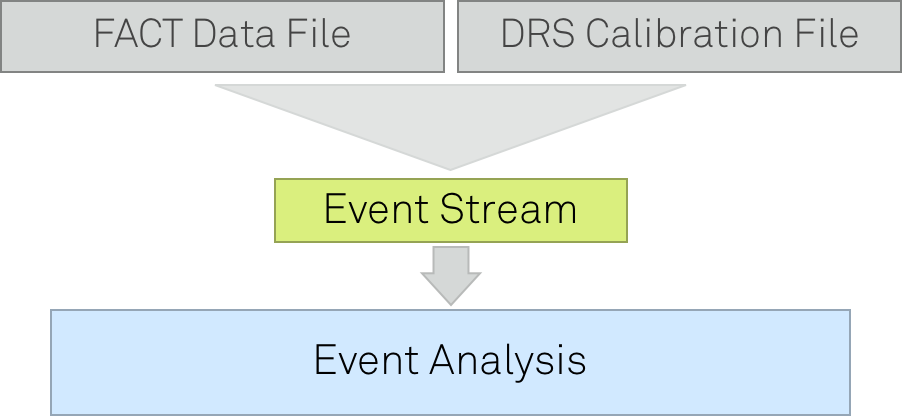
\includegraphics[scale=0.2]{fact-event-stream}
\end{center}
\caption{\label{fig:eventStream}Stream-lined processing of events.}
\end{figure}





\subsubsection{Reading FACT Data}
The {\em fact-tools} library is an extension of the \streams framework that
adds domain specific implementations such as stream-sources and specific 
processors to process FACT data stored in FITS files. These processors provide
the code for calibrating the data according to previously observed parameters,
allow for camera image analysis (image cleaning) or for extracting features
for subsequent analysis.

The XML snippet in Figure \ref{fig:readFACTxml} defines a simple process to
read raw data from a FITS file and apply a calibration step to transform that
data into correct values based upon previously recorded calibration parameters.

\begin{figure}[h!]
\begin{lstlisting}{language=XML}
    <container>
        <stream id="factData" url="file:/data/2011-09-13-004.fits.gz"
             class="fact.io.FACTEventStream" />
        <process input="factData">
             <fact.io.DrsCalibration file="/data/2011-09-13-001.fits.drs.gz" />
             <!--  add further processors here  -->
        </process>
    </container>
\end{lstlisting}
\caption{\label{fig:readFACTxml}Basic process definition for reading raw FACT data
and calibrating that data.}
\end{figure}

Each single event that is read from the event stream, contains the
full raw, calibrated measurements of the telescope. 
%As with all other
%data stream implementations, the {\em FactEventStream} emits a sequence
%of {\em data items}, each of which contains the data of a single FACT
%event.
The attributes of the data items reflect the image data, event
meta information and all other data that has been recorded during the
observation. Table \ref{tab:factEventKeys} lists all the attributes of
an event that are currently provided by the {\ttfamily FACTEventStream}
class.
\begin{table}[h!]
\renewcommand{\arraystretch}{1.25}
{\footnotesize
  \begin{center}
    \begin{tabular}{l|l} \hline
      \textsf{\textbf{Name (key)}} & \textsf{\textbf{Description}} \\ \hline \hline
      {\ttfamily EventNum} & The event number in the stream \\ \hline
      {\ttfamily TriggerNum} & The trigger number in the stream \\ \hline
      {\ttfamily TriggerType} & The trigger type that caused recording of the event \\ \hline
      {\ttfamily NumBoards} & \\ \hline
      {\ttfamily Errors} & \\ \hline
      {\ttfamily SoftTrig} & \\ \hline
      {\ttfamily UnixTimeUTC} & \\ \hline
      {\ttfamily BoardTime} & \\ \hline
      {\ttfamily StartCellData} & \\ \hline
      {\ttfamily StartCellTimeMarker} & \\ \hline
      {\ttfamily Data} & The raw data array ($1440\cdot 300 = 432000$ float values) \\ \hline
      {\ttfamily TimeMarker} & \\ \hline
      {\ttfamily @id} & A simple identifier providing date, run and event IDs \\ \hline
      {\ttfamily @source} & The file or URL the event has been read from \\ \hline
    \end{tabular}
  \end{center}}
  \caption{\label{tab:factEventKeys} The elements available for each event.}
\end{table}

The {\ttfamily @id} and {\ttfamily @source} attributes provide
meta-information that is added by the FACT-stream implementation
itself, all the other attributes are provided within the FITS data
files. The {\ttfamily @id} attribute's value is created from the
{\ttfamily EventNum} and date when the event was recorded,
e.g. {\ttfamily 2011/11/27/42/8}, denoting the event 8 in run 42 on
the 27th of November 2011.


\subsubsection{Processors for FACT Data}
Any of the existing core processors of the \streams library can directly be applied
to data items of the FACT event stream. This already allows for general applications
such as adding additional data (e.g. whether data from a database).

The {\em fact-tools} library provides several domain specific processors that focus
on the handling of FACT events. The {\ttfamily DrsCalibration} processor for calibrating
the raw data has already been mentioned above.

Other processors included are more specifically addressing the image-analysis task:
\begin{itemize}
  \item {\ttfamily fact.data.CutSlices} \\
  Which can be used to select a subset of the raw data array for only a excerpt of
  the region-of-interest\footnote{The {\em region of interest} is the length of the
  recorded time for each event, usually 300 nanoseconds, at most 1024 nanoseconds} (ROI).

  \item {\ttfamily fact.data.SliceNormalization} \\
  As there is a single-valued series of floats provided for each pixel, this processor
  allows for normalizing the values for these series to $[0,1]$.

  \item {\ttfamily fact.data.MaxAmplitude} \\
  This processor extracts a float-array of length 1440, which contains the maximum
  amplitude for each pixel.

  \item {\ttfamily fact.image.DetectCorePixel} \\
  This class implements a heuristic strategy to select the possible core-pixels of
  a shower, that may be contained within the event.
\end{itemize}


\subsection*{Installing the FACT-Plugin}
The FACT-Plugin is an extension for RapidMiner. The RapidMiner
open-source software is written in Java and is available for multiple
environments (Windows, Unix). It can be downloaded from
\url{http://rapid-i.com}.

The FACT-Plugin is a simple Java archive ({\em jar}-file) that can be
found at
\begin{displaymath}
 \mbox{\url{http://sfb876.tu-dortmund.de/FACT/}}
\end{displaymath}
To install the plugin simply copy the latest {\ttfamily FACT-Plugin.jar}
to your RapidMiner {\ttfamily lib/plugins} directory. After restarting
RapidMiner, the plugin will be loaded and all of its additional operators
will show up in the operators list.





%%%
%%
%%
\subsection{\label{sec:videoStreams}Processing Video Streams}
\baustelle The processing of video streams is a recent application
that has been added to the \streams framework. The {\em streams-video}
package provides an implementation for streams of video frames in the
MJPEG format.

Several procssors have been added, e.g. for the extraction of features
from online video data. Features from videos might e.g. be indicating
commercial breaks or switches in scenes. 
cannot be derived from static EPG data or any other annotating data
sources. An overview about the video processing and the associated
scene and shot detection is outlined in Section
\ref{sec:videoFeatures}.

Researching the feature extraction from video data focuses on image
analysis of single video frames and the derived stream of features from
a series of such frames. The static feature extraction from images is
being investigated with the RapidMiner Image Mining Plugin \cite{Burget2010a}.

To support the online feature extraction from video data, the TUDO
group provides an image stream implemented for the \streams framework
which allows for applying processors to video frames in a streaming
manner. A sample of process definition for reading RAW video streams
is shown in Figure \ref{fig:videoXml}.

\begin{figure}[h!]
  \centering
  \begin{lstlisting}
    <container>

        <!--  This stream reads encoded JPG images from a file       -->    
        <stream  id="video" class="stream.io.MJpegImageStream"
                url="file:/Volumes/RamDisk/tagesschau.mjpeg.stream" />

        <process input="video">
             <!--  Add a 'frame:id' attribute, counting the frames    -->
             <CreateID key="frame:id" />
        
             <!--  Extract the average RGB channel values             -->
             <vista.video.ExtractAverageRGB />

             <!--  Plot the average red/green/blue channel values     -->         
             <WithKeys keys="frame:*" >
                  <stream.plotter.Plotter keys="frame:red:avg,frame:blue:avg,frame:green:avg"
                                       history="1000" />
             </WithKeys>
        </process>
    </container>
  \end{lstlisting}
  \caption{\label{fig:videoXml}A process definition for reading RAW
    video files encoded as a sequence of JPEG images. The processors
    used in this sample allow for extracting the average R/G/B channel
    values for each frame. The result is a 3-dimensional time series,
    emitting data at the usual frame rate of 25 samples per second.}
\end{figure}

\subsubsection*{Decoding Videos to MJPEG}
The format required for the {\ttfamily MJpegImageStream}
implementation to read video frames is a file of RAW decoded video
frames in JPEG image format. The stream implementation does not do the
decoding itself. Such a decoding can easily be derived from the open
source {\em MPlayer} tool, which is available for Linux, MacOS and
Windows. The {\em MPlayer} tool provides a standalone video decoder
called {\ttfamily mencoder} that can decode video streams and encode
these into various formats, including RAW JPEG sequence files.

For decoding a file {\ttfamily tagesschau.mp4}\footnote{The {\em
    Tagesschau} is a German news show, which provides hourly summaries
  of 90 seconds length. These can be downloaded from
  \url{http://www.tagesschau.de} and are used here for demonstration
  only.}, the {\ttfamily mencoder} needs to be invoked as:
\begin{verbatim}
   # mencoder tagesschau.mp4 -nosound -of rawvideo -o tagesschau.raw \
        -ovc lavc -lavcopts vcodec=mjpeg
\end{verbatim}
This will write a RAW JPEG sequence file to {\ttfamily tagesschau.raw}
which in turn can be read with the {\ttfamily MJpegImageStream} as shown
in Figure \ref{fig:videoXml}.

The {\ttfamily MJpegImageStream} will provide data items that contain
the raw byte array of the JPEG image in the {\ttfamily image:data}
attribute. This can further be used by processors to decode the original
bitmap image or display the image. The processor {\ttfamily AverageRGB}
decodes the image to a bitmap in order to compute the average color
channel values for the complete frame.

The {\ttfamily mencoder} tool as well as the \streams framework support
reading from standard input and writing to standard output. This allows
for decoding and processing live video streams from the Zattoo platform
later on.


\begin{figure}[h!]
  \centering
  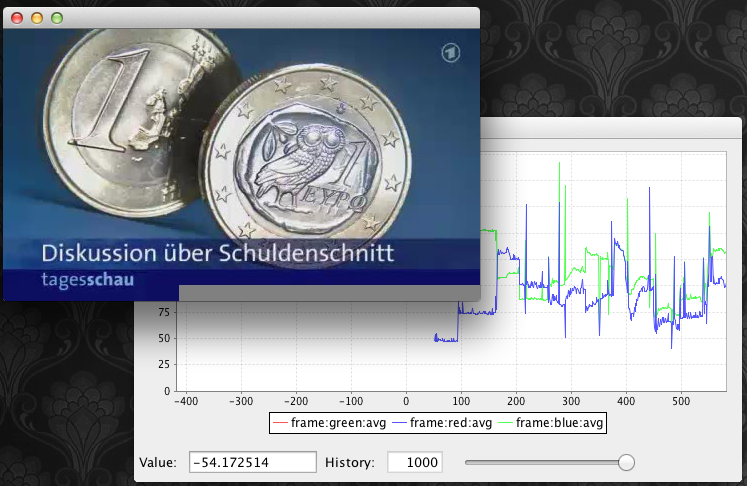
\includegraphics[scale=0.3]{graphics/video-stream.png}
  \caption{\label{fig:videoStreaming}The \streams framework
    continuously extracting average R/G/B channel values from a sample
    video while displaying the video frames to the screen.}
\end{figure}

%\subsection{Analyzing Log-File Streams}
%
%\subsection{Monitoring Steel-Production Processes}


%%
%% Section 7 Summary & Future Work
%%
%%
%%
%%
\section{\label{sec:summary}Summary and Future Work}
In this report we introduced the \streams framework, which provides
means for abstracting the definition of data flow graphs for data
stream processing. The level of abstraction provided by the \streams
framework enables a rapid prototyping of compute graphs for process
design as well as providing a simple programming API to include
custom functionality into the designed processes.

The use of XML for process/graph definitions supports a simple
exchange of designed processes between users and lifts the level of
detail for data analysists to hide implementation details where they
may be distracting from the process design task.

The \streams framework also provides a reference implementation for
running compute graphs on a single Java virtual machine as well as a
compiler for mapping graphs to topologies that execute on the {\em
  Storm} stream engine.

The integration of the {\em MOA} library adds various online learning
schemes to the \streams framework. This shows the applicability of the
proposed abstraction layer for the field of online learning. In addition
the \streams library proved to be useful in application use-cases like
pre-processing of the FACT telescope data or the coffee machine video
processing.

\bigskip

Ongoing work currently focuses on a more extensive integration of
additional algorithms provided by {\em MOA} (e.g. clustering). The
adaption of the \streams runtime for the Android platform has revealed
a prototype for running XML process definitions on mobile devices. This
is another direction that will be integrated into the next release of
the \streams framework.

For a more convenient design of \streams process definitions, we will
investigate different XML or process editors that can assist users in
rapid prototyping of data stream processes.

%%
%% Appendix (API, Installation,...)
%%
\part{API Documentation}
\begin{appendix}
\section{The \streams Core Classes}
The \streams framework provides a wide range of implementations for
data streams and processors. These are useful for reading application
data and defining a complete data flow.

In this section we provide a comprehensive overview of the classes and
implementations already available in the \streams library. These can
directly be used to design stream processes for various application
domains.

%\subsubsection{Package {\ttfamily stream.io}}
\subsection{\label{app:dataStreams}\label{api:stream:io}Data Stream Implementations}

Reading data is usually the first step in data processing. The package
{\ttfamily stream.io} provides a set of data stream implementations
for data files/resources in various formats.

All of the streams provided by this package do read from URLs, which
allows reading from files as well as from network URLs such as HTTP
urls or plain input streams (e.g. standard input).

The streams provide an iterative access to the data and use the default
\texttt{DataFactory} for creating data. They do usually share some
common parameters supported by most of the streams such as
\texttt{limit} or \texttt{username} and \texttt{password}.

\subsubsection*{Defining a Stream}
As discussed in Section \ref{sec:designingProcesses}, a stream is
defined within a container using the XML {\ttfamily stream} element,
providing a {\ttfamily url} and {\ttfamily class} attribute which
determines the source to read from and the class that should be used
for reading from that source. In addition, the definition requires a
third attribute {\ttfamily id}, which assigns the stream with a
(unique) identifier. This identifier is then used to reference the
stream as input to a process.

As a simple example, the following XML snippet defines a data stream
that reads data items in CSV format from some file URL:
\begin{figure}[h!]
        \centering
        \begin{lstlisting}{lang=xml}
           <stream  id="csv-data" class="stream.io.CsvStream"
                   url="file:/tmp/example.csv" />
        \end{lstlisting}
        \caption{Defining a CSV stream from a file.}
\end{figure}

\subsubsection*{Streaming Data from various URLs}
The \streams runtime supports a list of different URL schemes which
are provided by all Java virtual machines, e.g. {\ttfamily http} URLs
or {\ttfamily file} URLs. Custom URL schemes can also be registered
within the Java VM. As of this, the \streams runtime additionally
offers a {\ttfamily classpath:} and a {\ttfamily system:} URL scheme.

The {\ttfamily classpath:} URLs can be used to create data streams
that read from resources which are available on the classpath. This is
useful for providing example sources within custom JAR files or the
like. The following example shows how to create a stream that reads
data in JSON format from a resource {\ttfamily example.json} that is
searched for in the default classpath:
\begin{figure}[h!]
        \centering
        \begin{lstlisting}{lang=xml}
           <stream  id="json-stream"  class="stream.io.JSONStream"
                   url="classpath:/example.json" />
        \end{lstlisting}
        \caption{\label{fig:jsonStreamClasspath}Defining a JSON stream from a classpath resource.}
\end{figure}

To support streams that read data from standard input or standard
error, the library provides the {\ttfamily system:} URL schema. This
schema provides access to the system input and error streams and are
useful when piping data to a stream via the command line, e.g. by
running a command like:
\begin{figure}[h!]
\sample{\# cat data.csv | stream.run my-process.xml}
\end{figure}
To define a stream that reads from standard input, simply specify
{\ttfamily system:input} as the streams URL as shown in figure
\begin{figure}[h1]
        \centering
        \begin{lstlisting}{lang=xml}
           <stream  id="example"  class="stream.io.CsvStream"
                   url="system:input" />
        \end{lstlisting}
        \caption{\label{fig:csvStreamStdin}Defining a CSV stream that reads data from the system's standard input.}
\end{figure}

\newpage
\input{stream_io_ArffStream}

\input{stream_io_CsvStream}

\input{stream_io_JSONStream}
\input{stream_io_LineStream}
\input{stream_io_ProcessStream}
\input{stream_io_SQLStream}
\input{stream_io_SvmLightStream}
\input{stream_io_TimeStream}

\newpage
\subsection{\label{api:stream:queues}Queue Implementations}
The notion of queues is similar to the definition of streams within
the \streams framework. Queues provide can be attached as sources to
processes while also allowing to be fed with data items from other
places. This allows for simple inter-process communication by
forwarding data items from one process to the queue that is read by
another different process.



\input{stream_io_BlockingQueue}
%\input{stream_io_CsvUpload}
%\input{stream_io_CsvWriter}
%\input{stream_io_JSONWriter}
%\input{stream_io_LineWriter}
%\input{stream_io_ListDataStream}
%\input{stream_io_SQLWriter}
%\input{stream_io_SvmLightStream}
%\input{stream_io_SvmLightWriter}
%\input{stream_io_TimeStream}
%\input{stream_io_TreeStream}


\subsection{The {\em stream-core} Processor Classes}

\subsection{Package stream.flow}

The \texttt{stream.flow} package contains processors that allow for data
flow control within a process setup. Processors in this package are
usually processor-lists, i.e.~they may provide nested processors that
are executed based on conditions.

A typical example for control flow is given with the following
\texttt{If} processor, which executes the \texttt{PrintData} processor
only, if the value of attribute \texttt{x1} is larger than 0.5.

\begin{verbatim}
   <If condition="%{data.x1} @gt 0.5">
       <PrintData />
   </If>
\end{verbatim}
Other flow control processors provide control of data queues such as
enqueuing events into other processes' queues.


\input{stream_flow_CreateAndEnqueue}
\input{stream_flow_CreateAndMultiEnqueue}
\input{stream_flow_Delay}
\input{stream_flow_Enqueue}
\input{stream_flow_Every}
\input{stream_flow_If}
\input{stream_flow_MultiEnqueue}
\input{stream_flow_OnChange}
\input{stream_flow_Skip}


\Package{stream.data}
This package provides processors that perform transformations or
mangling of the data items themselves. Examples for such processors are
\texttt{CreateID}, which adds a sequential ID attribute to each
processed item or the \texttt{RemoveKeys} processor which removes
attributes by name.

Other useful processors provide numerical binning
(\texttt{NumericalBinning}), setting of values in various scopes
(\texttt{SetValue}) and the like.


%\input{stream_data_AddTimestamp}
%\input{stream_data_AsJSON}
%\input{stream_data_BinaryLabels}
%\input{stream_data_CreateID}
%\input{stream_data_Lookup}
%\input{stream_data_MapKeys}
%\input{stream_data_MapValueToID}
%\input{stream_data_MapValues}
%\input{stream_data_NumericalBinning}
%\input{stream_data_PrintData}
%\input{stream_data_RandomBinaryLabel}
%\input{stream_data_RemoveKeys}
%\input{stream_data_RemoveZeroes}
%\input{stream_data_RenameKey}
%\input{stream_data_SelectKeys}
%\input{stream_data_SetValue}
%\input{stream_data_TrimKeys}
\input{stream_data_WithKeys}

\subsection{Package stream.parser}

When processing streams of data each single data item may contain
additional information that needs to be extracted into more detailed
attributes or into other value types.

The \texttt{stream.parser} package provides a set of parsing processors,
that usually act upon on or more keys and extract information from the
attributes denoted by those keys.

For example the \texttt{ParseDouble} processor will parse double values
from all strings that are denoted in its \texttt{keys} parameter. Other
parsers in this package are for example the \texttt{ParseJSON},
\texttt{Timestamp} or the \texttt{NGrams} processor.


\input{stream_parser_NGrams}
\input{stream_parser_ParseDouble}
\input{stream_parser_ParseTimestamp}

\section{\label{sec:factAPI}Processors for FACT Data}
\section{\label{sec:streamsRuntime}The \streams Runtime}
Along with the \streams API, that is provided for implementing custom
streams or processors, the \streams framework provides a runtime
environment for running stream containers.

\subsection{Installing the \streams Runtime on Debian/RedHat}
For Debian and RPM based systems, there exists a package repository,
that provides Debian and RPM packages that can easily be installed
using the system's package managers. A step-by-step guide for setting
up the package manager on Debian and Ubuntu systems is provided in
Section \ref{sec:installDeb}. Instructions for RedHat based systems
such as RedHat, CentOS or Scientific Linux are provided in
\ref{sec:installRPM}.


\subsubsection{\label{sec:gpgKey}Signatures for Packages}
The repositories and all packages within the repository are
cryptographically signed with a GPG key with ID {\ttfamily 0x13443F4A}
to ensure their consistency. The key is available at

\sample{http://download.jwall.org/software.gpg}

The key is associated with the following information:

\sample{User ID: jwall.org Software Repository <software@jwall.org>\newline
Fingerprint: 175C 915F 51CA 8AA2 387B  E3E8 48E6 B98D 1344 3F4A}

This key needs to be added to the package management key ring of the
system (e.g. {\em apt} on Debian or {\em yum} on RedHat systems).

\subsubsection{\label{sec:installDeb}Installing on Debian/Ubuntu}
There exists a Debian/Ubuntu repository at {\ttfamily
  jwall.org}\footnote{The site \url{http://www.jwall.org/streams/} is
  the base web-site of the \streams framework.} which provides access
to the latest release versions of the \streams library.

To access this repository from within your Debian system, you'll need
create a new file {\ttfamily /etc/apt/sources.list.d/jwall.list} with
the following content:

\sample{ deb http://download.jwall.org/debian/ jwall main } 

The repositories and all packages within the repository are
cryptographically signed with a GPG key. Please see Section
\ref{sec:gpgKey} above for details on how to verify the correctness of
this key.

This key needs to be added to the APT key ring of the Debian/Ubuntu
system by running the following commands (the {\ttfamily \#} denotes
the shell prompt):

\sample{\# sudo wget http://download.jwall.org/debian/software.gpg\newline
\# sudo apt-key add software.gpg 
}

After the key and the repository have been added to the APT package
management, all that is left is to update the package list and install
the \streams environment with the following commands:

\sample{\# sudo apt-get update\newline
\# sudo apt-get install streams
}

The first command will update the package lists, the second will install
the lastest version of the {\ttfamily streams} package. After installation,
the system should be equipped with a new {\ttfamily stream.run} command
to run XML stream processes:

\sample{\# stream.run my-process.xml}

\subsubsection{\label{sec:installRPM}Installing on RedHat/CentOS/Fedora}
There exists a YUM repository at the {\ttfamily jwall.org} site, which
provides access to the latest release versions of the \streams framework
for RedHat based systems.

To access this repository from within your CentOS/RedHat system,
you'll need to create a file {\ttfamily /etc/yum.repos.d/jwall.repo}
with the following contents:

\sample{[jwall]\newline
name=CentOS-jwall - jwall.org packages for noarch\newline
baseurl=http://download.jwall.org/yum/jwall\newline
enabled=1\newline
gpgcheck=1\newline
protect=1}

The RPM packages are signed with a GPG key, please see Section
\ref{sec:gpgKey} for information how to validate this key.

To import the GPG key into your system's key ring, run the
following command as super user:

\sample{\# rpm --import http://download.jwall.org/software.gpg}

After the key has been imported your system is ready to install
the \streams package using the system's package manager, e.g.
by running

\sample{\# yum install streams}

This will download the required packages and set up the system
to provide the {\ttfamily stream.run} command to execute XML
stream processes.
\end{appendix}

%\section{\label{sec:Outlook}Conclusion and Future Work}
In this work we presented a simple abstraction API for modelling
continuous streaming processes and implementing custom processors and
services. On top of this layer of abstraction we implemented a
RapidMiner \plugin\  that integrates the stream oriented processing into
the RapidMiner suite. This allows for processing of continuous data or
large batch data sets using sequential single item or mini batch
processing.
%
%The API is simple to extend and new operators can easily be integrated
%by following ...
%
%\medskip

Future work will focus on integrating MOA into the \streams library,
making more data mining algorithms available for online processing. In
addition we seek for extending the remote access for other web service
protocols like SOAP. An interesting extension will be the integration
of distribution capabilities, e.g. by incorporating support for
backend infrastuctures like Twitter's {\em Storm} framework.

\paragraph{Acknowledgements} This work was supported by the DFG within
the Collaborative Research Center on {\em Providing Information by
  Resource-Constrained Data Analysis} (SFB-876).



% Bibliography using Bibtex, style plain
\bibliographystyle{plain}
\bibliography{literatur,local-refs}


\end{document}
